\chapter{Holomorphic functions}
Throughout this chapter, we denote by $U$ an open subset of the complex plane,
and by $\Omega$ an open subset which is also simply connected.
The main references for this chapter were \cite{ref:dartmouth,ref:bak_ca}.

\section{The nicest functions on earth}
In high school you were told how to differentiate and integrate real-valued functions.
In this chapter on complex analysis,
we'll extend it to differentiation and integration of complex-valued functions.

Big deal, you say. Calculus was boring enough. Why do I care about complex calculus?

Perhaps it's easiest to motivate things if I compare real analysis to complex analysis.
In real analysis, your input lives inside the real line $\RR$.
This line is not terribly discerning -- you can construct a lot of unfortunate functions.
Here are some examples.
\begin{example}
	[Optional: evil real functions]
	You can skim over these very quickly: they're just here to make a point.
	\begin{enumerate}[(a)]
		\ii The \vocab{Devil's Staircase} (or Cantor function)
		is a continuous function $H : [0,1] \to [0,1]$
		which has derivative zero ``almost everywhere'',
		yet $H(0) = 0$ and $H(1) = 1$.
		\ii The \vocab{Weierstra\ss\ function}
		\[ x \mapsto \sum_{n=0}^\infty \left( \half \right)^n \cos \left( 2015^n \pi x \right) \]
		is continuous \emph{everywhere} but differentiable \emph{nowhere}.
		\ii The function
		\[
			x \mapsto 
			\begin{cases}
				x^{100} & x \ge 0 \\
				-x^{100} & x < 0
			\end{cases}
		\]
		has the first $99$ derivatives but not the $100$th one.
		\ii
		If a function has all derivatives (we call these \vocab{smooth} functions),
		then it has a Taylor series.
		But for real functions that Taylor series might still be wrong. The function
		\[ x \mapsto
			\begin{cases}
				e^{-1/x} & x > 0 \\
				0 & x \le 0
			\end{cases}
		\]
		has derivatives at every point.
		But if you expand the Taylor series at $x=0$, you get $0 + 0x + 0x^2 + \dots$,
		which is wrong for \emph{any} $x > 0$ (even $x=0.0001$).
	\end{enumerate}
\end{example}
\begin{figure}[h]
	\centering
	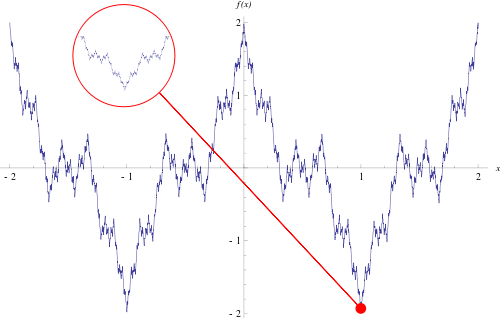
\includegraphics[width=0.8\textwidth]{media/weierstrass-pubdomain.png}
	\caption{The Weierstra\ss\ Function (image from \cite{img:weierstrass}).}
\end{figure}

Let's even put aside the pathology.
If I tell you the value of a real smooth function on the interval $[-1, 1]$,
that still doesn't tell you anything about the function as a whole.
It could be literally anything, because it's somehow possible to ``fuse together'' smooth functions.

So what about complex functions?
If you just consider them as functions $\RR^2 \to \RR^2$, you now have the interesting property
that you can integrate along things that are not just line segments: you can write integrals
across curves in the plane.
But $\CC$ has something more: it is a \emph{field}, so you can \emph{multiply} and \emph{divide} two complex numbers.

So we restrict our attention to differentiable functions called \emph{holomorphic functions}.
It turns out that the multiplication on $\CC$ makes all the difference.
The primary theme in what follows is that holomorphic functions are \emph{really, really nice},
and that knowing tiny amounts of data about the function can determine all its values.
%In particular, they are highly \emph{rigid} and \emph{regular}.

The two main highlights of this chapter,
from which all other results are more or less corollaries:
\begin{itemize}
	\ii Contour integrals of loops are always zero.
	\ii A holomorphic function is essentially given by its Taylor series;
	in particular, single-differentiable implies infinitely differentiable.
	Thus, holomorphic functions behave quite like polynomials.
\end{itemize}
Some of the resulting corollaries:
\begin{itemize}
	\ii It'll turn out that knowing just the values of a holomorphic function
	on the boundary of the unit circle will tell you the values in its interior.
	\ii Knowing just the values of the function at $1$, $\half$, $\frac13$, \dots
	are enough to determine the whole function!
	\ii Bounded holomorphic functions $\CC \to \CC$ must be constant
	\ii And more\dots
\end{itemize}

As \cite{ref:pugh} writes: ``Complex analysis is the good twin and real analysis is the evil one: beautiful formulas and elegant theorems seem to blossom spontaneously in the complex domain, while toil and pathology rule the reals''.


\section{Complex differentiation}
\prototype{Polynomials are holomorphic; $\ol z$ is not.}
Let $f : U \to \CC$ be a complex function.
Then for some $z_0 \in U$, we define the \vocab{derivative} at $z_0$ to be
\[
	\lim_{h \to 0} \frac{f(z_0+h) - f(z_0)}{h}.
\]
Note that this limit may not exist; when it does we say $f$ is \vocab{differentiable} at $z_0$.

What do I mean by a ``complex'' limit $h \to 0$?
It's what you might expect: for every $\eps > 0$ there should be a $\delta > 0$
such that 
\[ 0 < \left\lvert h \right\rvert < \delta
	\implies
	\left\lvert \frac{f(z_0+h)-f(z_0)}{h} - L \right\rvert < \eps. \]
If you like topology, you are encouraged to think of this in terms of neighborhoods in the complex plane.
(This is why we require $U$ to be open: it makes it possible to take $\delta$-neighborhoods in it.)

But note that having a complex derivative is actually much stronger
than a real function having a derivative.
In the real line, $h$ can only approach zero from below and above,
and for the limit to exist we need the ``left limit'' to equal the ``right limit''.
But the complex numbers form a \emph{plane}: $h$ can approach zero
from many directions, and we need all the limits to be equal.

\begin{example}
	[Important: conjugation is \emph{not} holomorphic]
	Let $f(z) = \ol z$ be complex conjugation, $f : \CC \to \CC$.
	This function, despite its simple nature, is not holomorphic!
	Indeed, at $z=0$ we have,
	\[ \frac{f(h)-f(0)}{h} = \frac{\ol h}{h}. \]
	This does not have a limit as $h \to 0$, because depending
	on ``which direction'' we approach zero from we have different values.
	\begin{center}
		\begin{asy}
			size(7cm);
			dot("$0$", origin, dir(225));
			void meow(string s, real theta, real eps = 45, pen p) {
				draw( (dir(theta) * 0.8) -- (dir(theta) * 0.2), p+1);
				draw( (dir(theta) * 0.8) -- (dir(theta) * 0.2), p, Arrow);
				label(s, dir(theta)*0.5, dir(eps), p);
			}
			meow("$1$", 0, 90, blue);
			meow("$1$", 180, 90, blue);
			meow("$i$", -45, 45, heavygreen);
			meow("$-1$", 90, 0, red);
			label("$f(z) = \overline z$", dir(135));
			label("$\dfrac{f(0+h)-f(0)}{h}$", dir(135)-0.35*dir(90));

			import graph;
			graph.xaxis("Re", -1, 1, grey, NoTicks, Arrows);
			graph.yaxis("Im", -1, 1, grey, NoTicks, Arrows);
		\end{asy}
	\end{center}
\end{example}

If a function $f : U \to \CC$ is complex differentiable
at all the points in its domain it is called \vocab{holomorphic}.
In the special case of a holomorphic function with domain $U = \CC$,
we call the function \vocab{entire}.\footnote{Sorry, I know the word ``holomorphic'' sounds so much cooler. I'll try to do things more generally for that sole reason.}

\begin{example}
	[Examples of holomorphic functions]
	In all the examples below, the derivative of the function
	is the same as in their real analogues
	(e.g.\ the derivative of $e^z$ is $e^z$).
	\begin{enumerate}[(a)]
		\ii Any polynomial $z \mapsto z^n + c_{n-1} z^{n-1} + \dots + c_0$ is holomorphic.
		\ii The complex exponential $\exp : x+yi \mapsto e^x (\cos y + i \sin y)$
		can be shown to be holomorphic.
		\ii $\sin$ and $\cos$ are holomorphic when extended
		to the complex plane by $\cos z = \frac{e^{iz}+e^{-iz}}{2}$
		and $\sin z = \frac{e^{iz}-e^{-iz}}{2}$.
		\ii As usual, the sum, product, chain rules and so on apply,
		and hence \textbf{sums, products, nonzero quotients,
		and compositions of holomorphic functions are also holomorphic}.
	\end{enumerate}
\end{example}
You are welcome to try and prove these results, but I won't bother to do so.

\section{Contour integrals}
\prototype{$\oint_\gamma z^m \; dz$ around the unit circle.}
In the real line we knew how to integrate a function across a line segment $[a,b]$:
essentially, we'd ``follow along'' the line segment adding up the values of $f$ we see
to get some area.
Unlike in the real line, in the complex plane we have the power to integrate
over arbitrary paths: for example, we might compute an integral around a unit circle.
A contour integral lets us formalize this.

First of all, if $f : \RR \to \CC$ and $f(t) = u(t) + iv(t)$ for $u,v \in \RR$,
we can define an integral $\int_a^b$ by just adding the real and imaginary parts:
\[ \int_a^b f(t) \; dt
	= \left( \int_a^b u(t) \; dt \right)
	+ i \left( \int_a^b v(t) \; dt \right). \]
Now let $\alpha : [a,b] \to \CC$ be a path, thought of as
a complex differentiable\footnote{This isn't entirely correct here:
	you want the path $\alpha$ to be continuous and mostly differentiable,
	but you allow a finite number of points to have ``sharp bends''; in other words,
	you can consider paths which are combinations of $n$ smooth pieces.
	But for this we also require that $\alpha$ has ``bounded length''.} function.
Such a path is called a \vocab{contour},
and we define its \vocab{contour integral} by
\[
	\oint_\alpha f(z) \; dz
	= \int_a^b f(\alpha(t)) \cdot \alpha'(t) \; dt.
\]
You can almost think of this as a $u$-substitution (which is where the $\alpha'$ comes from).
In particular, it turns out this integral does not depend on how $\alpha$ is ``parametrized'':
a circle given by \[ [0,2\pi] \to \CC : t \mapsto e^{it} \]
and another circle given by \[ [0,1] \to \CC : t \mapsto e^{2\pi i t} \]
and yet another circle given by \[ [0,1] \to \CC : t \mapsto e^{2 \pi i t^5} \]
will all give the same contour integral, because the paths they represent have the same
geometric description: ``run around the unit circle once''.

In what follows I try to use $\alpha$ for general contours and $\gamma$ in the special case of loops.

Let's see an example of a contour integral.
\begin{theorem}
	\label{thm:central_cauchy_computation}
	Take $\gamma : [0,2\pi] \to \CC$ to be the unit circle specified by 
	\[ t \mapsto e^{it}. \]
	Then for any integer $m$, we have
	\[ \oint_\gamma z^{m} \; dz
		=
		\begin{cases}
			2\pi i & m = -1 \\
			0 & \text{otherwise}
		\end{cases}
		\]
\end{theorem}
\begin{proof}
	The derivative of $e^{it}$ is $i e^{it}$.
	So, by definition the answer is the value of
	\begin{align*}
		\int_0^{2\pi} (e^{it})^m \cdot (ie^{it}) \; dt
		&= \int_0^{2\pi} i(e^{it})^{1+m} \; dt \\
		&= i \int_0^{2\pi} \cos [(1+m)t] + i \sin [(1+m)t] \; dt \\
		&= - \int_0^{2\pi} \sin [(1+m)t] \; dt + i \int_0^{2\pi} \cos [(1+m)t] \; dt.
	\end{align*}
	This is now an elementary calculus question.
	One can see that this equals $2\pi i$ if $m=-1$ and
	otherwise the integrals vanish.
\end{proof}
Let me try to explain why this intuitively ought to be true for $m=0$.
In that case we just have $\oint_\gamma 1 \; dz$.
So as the integral walks around the unit circle, it ``sums up'' all the tangent vectors
at every point (that's the direction it's walking in), multiplied by $1$.
And given the nice symmetry of the circle, it should come as no surprise that everything cancels out.
The theorem says that even if we multiply by $z^m$ for $m \neq -1$, we get the same cancellation.

\begin{center}
	\begin{asy}
		size(5cm);
		draw(unitcircle, dashed);
		void arrow(real theta) {
			pair P = dir(theta);
			dot(P);
			pair delta = 0.4*P*dir(90);
			draw( P--(P+delta), EndArrow );
		}
		arrow(0);
		arrow(50);
		arrow(140);
		arrow(210);
		arrow(300);
	\end{asy}
\end{center}

\begin{definition}
	Given $\alpha : [0,1] \to \CC$,
	we denote by $\ol\alpha$ the ``backwards'' contour
	$\ol\alpha(t) = \alpha(1-t)$.
\end{definition}

\begin{ques}
	What's the relation between $\oint_\alpha f \; dz$ and $\oint_{\ol\alpha} f \; dz$?
	Prove it.
\end{ques}

This might seem a little boring.
Things will get really cool really soon, I promise.

\section{Cauchy-Goursat theorem}
\prototype{$\oint_\gamma z^m \; dz = 0$ for $m \ge 0$. But if $m < 0$, Cauchy's theorem does not apply.}
Let $\Omega \subseteq \CC$ be simply connected (for example, $\Omega = \CC$),
and consider two paths $\alpha$, $\beta$ with the same start and end points.

\begin{center}
	\begin{asy}
		unitsize(0.8cm);
		bigbox("$\Omega$");
		pair A = Drawing((-3,0));
		pair B = Drawing((3,0));
		draw(A..(-2,0.5)..MP("\alpha", (0,2), dir(90))..(1,1.2)..B, red, EndArrow);
		draw(A----MP("\beta", (A+B)/2, dir(-90))--B, blue, EndArrow);
	\end{asy}
\end{center}

What's the relation between $\oint_\alpha f(z) \; dz$ and $\oint_\beta f(z) \; dz$?
You might expect there to be some relation between them, considering that the space $\Omega$ is simply connected.
But you probably wouldn't expect there to be \emph{much} of a relation.

As a concrete example, let $\Psi : \CC \to \CC$ be the function $z \mapsto z - \Re[z]$
(for example, $\Psi(2015+3i) = 3i$). Let's consider two paths from $-1$ to $1$.
Thus $\beta$ just walking along the real axis, and $\alpha$ which follows an upper semicircle.

\begin{center}
	\begin{asy}
		pair A = Drawing("-1", dir(180), dir(-90));
		pair B = Drawing("1", dir(0), dir(-90));
		draw(arc(origin, 1, 180, 0), red, EndArrow);
		MP("\alpha", dir(90), dir(90));
		draw(A--B, blue, EndArrow);
		MP("\beta", 0, dir(-90));
	\end{asy}
\end{center}

Obviously $\oint_\beta \Psi(z) \; dz = 0$.
But heaven knows what $\oint_\alpha \Psi(z) \; dz$ is supposed to equal.
We can compute it now just out of non-laziness.
If you like, you are welcome to compute it yourself (it's a little annoying but not hard).
If I myself didn't mess up, it is
\[ \oint_\alpha \Psi(z) \; dz = - \oint_{\ol\alpha} \Psi(z) \; dz
= - \int_0^\pi (i \sin(t)) \cdot ie^{it} \; dt = \half\pi i \]
which in particular is not zero.

But somehow $\Psi$ is not a really natural function.
It's not respecting any of the nice, continuous structure of $\CC$ since
it just rudely lops off the real part of its inputs.
More precisely,
\begin{ques}
	Show that $\Psi(z) = z - \Re[z]$ is not holomorphic.
	(Hint: $\ol z$ is not holomorphic.)
\end{ques}

Now here's a miracle: for holomorphic functions, the two integrals are \emph{always equal}.
Equivalently, (by considering $\alpha$ followed by $\ol\beta$) contour integrals of loops are always zero.
This is the celebrated Cauchy-Goursat theorem
(also called the Cauchy integral theorem,
but later we'll have a ``Cauchy Integral Formula'' so blah).

\begin{theorem}
	[Cauchy-Goursat theorem]
	Let $\gamma$ be a loop, and $f : \Omega \to \CC$ a holomorphic function
	where $\Omega$ is open in $\CC$ and simply connected.
	Then
	\[ \oint_\gamma f(z) \; dz = 0. \]
\end{theorem}
\begin{remark}[Sanity check]
	This might look surprising considering that we saw $\oint_\gamma z^{-1} \; dz = 2 \pi i$ earlier.
	The subtlety is that $z^{-1}$ is not even defined at $z = 0$.
	On the other hand, the function $\CC \setminus \{0\} \to \CC$ by $z \mapsto \frac 1z$ \emph{is} holomorphic!
	The defect now is that $\Omega = \CC \setminus \{0\}$ is not simply connected.
	So the theorem passes our sanity checks, albeit just barely.
\end{remark}

The typical proof of Cauchy's Theorem assumes additionally
that the partial derivatives of $f$ are continuous
and then applies the so-called Green's theorem.
But it was Goursat who successfully proved the fully general theorem we've stated above,
which assumed only that $f$ was holomorphic.
I'll only outline the proof, and very briefly.
You can show that if $f : \Omega \to \CC$ has an antiderivative $F : \Omega \to \CC$ which is also holomorphic,
and moreover $\Omega$ is simply connected, then you get a ``fundamental theorem of calculus'', a la
\[ \oint_\alpha f(z) \; dz = F(\alpha(b)) - F(\alpha(a)) \]
where $\alpha : [a,b] \to \CC$ is some path.
So to prove Cauchy-Gorsat, you just have to show this antiderivative $F$ exists.
Goursat works very hard to prove the result in the special case that $\gamma$ is a triangle,
and hence by induction for any polygon.
Once he has the result for a rectangle, he uses this special case to construct the function $F$ explicitly.
Goursat then shows that $F$ is holomorphic, completing the proof.

Anyways, the theorem implies that $\oint_\gamma z^m \; dz = 0$ when $m \ge 0$.
So much for all our hard work earlier.
But so far we've only played with circles.
This theorem holds for \emph{any} contour which is a loop.
So what else can we do?

\section{Cauchy's integral theorem}
We now present a stunning application of Cauchy-Gorsat, a ``representation theorem'':
essentially, it says that values of $f$ inside a disk
are determined by just the values on the boundary!
In fact, we even write down the exact formula.
As \cite{ref:dartmouth} says,
``any time a certain type of function satisfies some sort of representation theorem,
it is likely that many more deep theorems will follow.''
Let's pull back the curtain:

\begin{theorem}[Cauchy's integral formula]
	Let $\gamma : [0,2\pi] \to \CC$ be a circle in the plane given by $t \mapsto Re^{it}$,
	which bounds a disk $D$.
	Suppose $f : U \to \CC$ is holomorphic such that $U$ contains the circle and its interior.
	Then for any point $a$ in the interior of $D$, we have
	\[ 
		f(a)
		=
		\frac{1}{2\pi i} \oint_\gamma \frac{f(z)}{z-a} \; dz.
	\]
\end{theorem}
Note that we don't require $U$ to be simply connected, but the reason is pretty silly:
we're only going to ever integrate $f$ over $D$, which is an open disk, and hence the disk
is simply connected anyways.

The presence of $2\pi i$, which you saw earlier in the form $\oint_{\text{circle}} z^{-1} \; dz$,
is no accident.
In fact, that's the central result we're going to use to prove the result.

\begin{proof}
	There are several proofs out there, but I want to give the one that really
	draws out the power of Cauchy's theorem. Here's the picture we have:
	there's a point $a$ sitting inside a circle $\gamma$,
	and we want to get our hands on the value $f(a)$.
	\begin{center}
		\begin{asy}
			size(3cm);
			draw(unitcircle, dashed, MidArrow);
			MP("\gamma", dir(-45), dir(-45));
			pair a = 0.1 * dir(60);
			dot("$a$", a, dir(a));
		\end{asy}
	\end{center}
	We're going to do a trick: construct a \vocab{keyhole contour} $\Gamma_{\delta, \eps}$
	which has an outer circle $\gamma$, plus an inner circle $\ol{\gamma_\eps}$, which is a circle centered
	at $a$ with radius $\eps$, running clockwise (so that $\gamma_\eps$ runs counterclockwise).
	The ``width'' of the corridor is $\delta$. See picture:
	\begin{center}
		\begin{asy}
			size(4cm);
			MP("\gamma", dir(-45), dir(-45));
			pair a = 0.1 * dir(60);
			dot("$a$", a, dir(a));
			real delta_outer = 6;
			real delta_inner = 20;
			pair P = dir(60+delta_outer);
			pair Q = dir(60-delta_outer);
			draw(arc(origin, 1, 60+delta_outer, 360+60-delta_outer), MidArrow);
			draw(arc(a, 0.3, 60-delta_inner, -360+60+delta_inner), MidArrow);
			draw(dir(60-delta_outer)--(a+0.3*dir(60-delta_inner)), MidArrow);
			draw((a+0.3*dir(60+delta_inner))--dir(60+delta_outer), MidArrow);
			MP("\overline{\gamma_\varepsilon}", a+0.3*dir(225), dir(225));
		\end{asy}
	\end{center}
	Hence $\Gamma_{\delta,\eps}$ consists of four smooth curves.
	\begin{ques}
		Draw a \emph{simply connected} open set $\Omega$ which contains the entire
		$\Gamma_{\delta,\eps}$ but does not contain the point $a$.
	\end{ques}
	Hence, the function $\frac{f(z)}{z-a}$ manages to be holomorphic on all of $\Omega$.
	Thus Cauchy's theorem applies and tells us that
	\[
		0 = \oint_{\Gamma_{\delta,\eps}} \frac{f(z)}{z-a} \; dz.
	\]
	As we let $\delta \to 0$, the two walls of the keyhole will cancel each other (because $f$ is continuous,
	and the walls run in opposite directions).
	So taking the limit as $\delta \to 0$, we are left with just $\gamma$ and $\gamma_\eps$, 
	which (taking again orientation into account) gives
	\[
		\oint_{\gamma} \frac{f(z)}{z-a} \; dz
		= - \oint_{\ol{\gamma_\eps}} \frac{f(z)}{z-a} \; dz
		= \oint_{\gamma_\eps} \frac{f(z)}{z-a} \; dz.
	\]
	Thus \textbf{we've managed to replace $\gamma$ with a much smaller circle $\gamma_\eps$ centered around $a$},
	and the rest is just algebra.

	To compute the last quantity, write
	\begin{align*}
		\oint_{\gamma_\eps} \frac{f(z)}{z-a} \; dz
		&=
		\oint_{\gamma_\eps} \frac{f(z)-f(a)}{z-a} \; dz
		+
		f(a) \cdot \oint_{\gamma_\eps} \frac{1}{z-a} \; dz \\
		&=
		\oint_{\gamma_\eps} \frac{f(z)-f(a)}{z-a} \; dz
		+
		2\pi i f(a).
	\end{align*}
	where we've used \Cref{thm:central_cauchy_computation}
	Thus, all we have to do is show that 
	\[ \oint_{\gamma_\eps} \frac{f(z)-f(a)}{z-a} \; dz = 0. \]
	For this we can basically use the weakest bound possible, the so-called $ML$ lemma
	which I'll just cite without proof:
	it just says ``bound the function everywhere by its maximum''.
	\begin{lemma}
		[$ML$ estimation lemma]
		Let $f$ be a holomorphic function and $\alpha$ a path.
		Suppose $M = \max_{z \text{ on } \alpha} \left\lvert f(z) \right\rvert$, and
		let $L$ be the length of $\alpha$.
		Then
		\[ \left\lvert \oint_\alpha f(z) \; dz \right\rvert \le ML. \]
	\end{lemma}
	(This is straightforward to prove if you know the definition of length:
	$L = \int_a^b \alpha'(t) \; dt$, where $\alpha : [a,b] \to \CC$.)

	Anyways, as $\eps \to 0$, the quantity $\frac{f(z)-f(a)}{z-a}$ just approaches $f'(a)$,
	and so for small enough $\eps$ (i.e.\ $z$ close to $a$) there's some upper bound $M$.
	Yet the length of $\gamma_\eps$ is just the circumference $2\pi \eps$.
	So the $ML$ lemma says that
	\[ \left\lvert \oint_{\gamma_\eps} \frac{f(z)-f(a)}{z-a} \right\rvert
		\le 2\pi\eps \cdot M \to 0
	\]
	as desired.
\end{proof}

\section{Holomorphic functions are analytic}
\prototype{Imagine a formal series $\sum_k c_kx^k$!}
In the setup of the previous problem, we have a circle $\gamma : [0,2\pi] \to \CC$
and a holomorphic function $U \to \CC$ which contains the disk $D$.
We can write
\begin{align*}
	f(a) &= \frac{1}{2\pi i} \oint_\gamma \frac{f(z)}{z-a} \; dz \\
	&= \frac{1}{2\pi i} \oint_\gamma \frac{f(z)/z}{1 - \frac az} \; dz \\
	&= \frac{1}{2\pi i} \oint_\gamma f(z)/z \cdot \sum_{k \ge 0} \left( \frac az \right)^k \; dz \\
	\intertext{You can prove (using the so-called Weierstrass M-test) that the summation order can be switched:}
	&= \frac{1}{2\pi i} \sum_{k \ge 0} \oint_\gamma \frac{f(z)}{z} \cdot \left( \frac az \right)^k \; dz \\
	&= \frac{1}{2\pi i} \sum_{k \ge 0} \oint_\gamma a^k \cdot \frac{f(z)}{z^{k+1}} \; dz \\
	&=  \sum_{k \ge 0} \left( \frac{1}{2\pi i}\oint_\gamma \frac{f(z)}{z^{k+1}} \; dz \right) a^k \\
	\intertext{Letting $c_k =  \frac{1}{2\pi i}\oint_\gamma \frac{f(z)}{z^{k+1}} \; dz$, and noting
this is independent of $a$, this is}
	&=  \sum_{k \ge 0} c_k a^k
\end{align*}
and that's the miracle: holomorphic functions are given by a Taylor series!
This is one of the biggest results in complex analysis.
Moreover, we also know that \[ c_k = \frac{f^{(k)}(0)}{k!} \] from AP Calculus (if you don't see this,
just take the derivative $k$ times), and this gives us $f^{(k)}(0) = k! \cdot c_k$.

Naturally, we can do this with any circle (not just one centered at zero).
So let's state the full result below, with arbitrary center $p$.

\begin{theorem}
	[Cauchy's differentiation formula]
	Let $f : U \to \CC$ be a holomorphic function and let $D$ be a disk centered at point $p$
	bounded by a circle $\gamma$.  Suppose $D$ is contained inside $U$.
	Then $f$ is given everywhere in $D$ by a Taylor series
	\[ 
		f(z) = c_0 + c_1(z-p) + c_2(z-p)^2 + \dots
	\]
	where
	\[
		c_k = \frac{f^{k}(p)}{k!} = \frac{1}{2\pi i} \oint_\gamma \frac{f(w-p)}{(w-p)^{k+1}} \; dw
	\]
	In particular, 
	\[ f^{(k)}(p) = k! c_k = \frac{k!}{2\pi i} \oint_\gamma \frac{f(w-p)}{(w-p)^{k+1}} \; dw. \]
\end{theorem}

Most importantly,
\begin{moral}
	Over any disk,
	a holomorphic function is given
	exactly by a Taylor series.
\end{moral}
This establishes a result we stated at the beginning of the chapter:
that a function being complex differentiable once means it is not only infinitely differentiable,
but in fact equal to its Taylor series.

I should maybe emphasize a small subtlety of the result:
the Taylor series centered at $p$ is only valid in a disk centered at $p$ which lies entirely in the domain $U$.
If $U = \CC$ this is no issue, since you can make the disk big enough to accommodate any point you want.
It's more subtle in the case that $U$ is, for example, a square; you can't cover the entire square
with a disk centered at some point without going outside the square.
However, since $U$ is open we can at any rate at least find some neighborhood for which the Taylor
series is correct -- in stark contrast to the real case.
Indeed, as you'll see in the problems,
the existence of a Taylor series is incredibly powerful.

\section\problemhead
These aren't olympiad problems, but I think they're especially nice!
In the next complex analysis chapter we'll see some more nice applications.

The first few results are the most important.


\begin{sproblem}
	[Liouville's theorem]
	\gim
	Let $f : \CC \to \CC$ be an entire function.
	Suppose that $\left\lvert f(z) \right\rvert < 1000$ for all complex numbers $z$.
	Prove that $f$ is a constant function.
	\begin{hint}
		Look at the Taylor series of $f$,
		and use Cauchy's differentiation formula to
		show that each of the larger coefficients must be zero.
	\end{hint}
%	\footnote{%
%	It's true more generally that if
%	$\left\lvert f(z) \right\rvert < A+B\left\lvert z \right\rvert^n$
%	for some constants $A$ and $B$,
%	then $f$ is a polynomial of degree at most $n$.
%	The proof is just induction on $n$ with the case $n=0$ being the theorem.}
\end{sproblem}


\begin{sproblem}[Zeros are isolated]
	An \vocab{isolated set} in the complex plane is a set of points $S$ such that
	around each point in $S$, one can draw a neighborhood not intersecting any other point of $S$.

	Show that the zero set of any nonzero holomorphic function $f : U \to \CC$
	is an isolated set, unless there exists a neighborhood of $f$ which is identically zero.
	\begin{hint}
		Proceed by contradiction, meaning there exists a sequence $z_1, z_2, \dots \to z$
		where $0 = f(z_1) = f(z_2) = \dots$ all distinct.
		Prove that $f = 0$ on some small neighborhood and apply the identity theorem.
	\end{hint}
	\begin{sol}
		Proceed by contradiction, meaning there exists a sequence $z_1, z_2, \dots \to z$
		where $0 = f(z_1) = f(z_2) = \dots$ all distinct.
		WLOG set $z=0$.
		Look at the Taylor series of $f$ around $z=0$.
		Since it isn't uniformly zero by assumption, write it as $a_Nz^N + a_{N+1}z^{N+1} + \dots$, $a_N \neq 0$.
		But by continuity of $h(z) = a_N + a_{N+1}z + \dots$ there is some
		neighborhood of zero where $h(z) \neq 0$.
	\end{sol}
\end{sproblem}

\begin{sproblem}
	[Identity theorem]
	\gim
	Let $f, g : U \to \CC$ be holomorphic, and assume that $U$ is connected.
	Prove that if $f$ and $g$ agree on some small neighborhood, then $f = g$.
	\begin{hint}
		Take the interior of the agreeing points;
		show that this set is closed, which implies the conclusion.
	\end{hint}
	\begin{sol}
		Let $S$ be the interior of the points satisfying $f=g$.
		By definition $S$ is open.
		By the previous part, $S$ is closed: if $z_i \to z$ and $z_i \in S$,
		then $f=g$ in some neighborhood of $z$, hence $z \in S$.
		Since $S$ is clopen and nonempty, $S = U$.
	\end{sol}
\end{sproblem}

\begin{figure}[ht]
	\centering
	\snsd[height=6cm]{bounded-like-complex-sine.jpg}
	\caption{Complex functions are unbounded. (Source: \cite{img:snsd}.)}
\end{figure}


%\begin{dproblem}
%	[Mean Value Property]
%	Let $f : U \to \CC$ be holomorphic.
%	Assume that $z_0 \in U$ and the disk centered at $z_0$
%	with radius $r > 0$ is contained inside $U$. Show that
%	\[ f(z_0) = \frac{1}{2\pi} \int_0^{2\pi} f(z_0+re^{it}) \; dt. \]
%	In other words, $f(z_0)$ is the average of $f$ along the circle.
%	\begin{hint}
%		Evaluate $\oint_\gamma \frac{f(w)}{w-z_0} \; dw$ over the circle.
%	\end{hint}
%\end{dproblem}

\begin{dproblem}[Maximums Occur On Boundaries]
	Let $f : U \to \CC$ be holomorphic, let $Y \subseteq U$ be compact,
	and let $\partial Y$ be boundary\footnote{
		The boundary $\partial Y$ is the set of points $p$
		such that no open neighborhood of $p$ is contained in $Y$.
		It is also a compact set if $Y$ is compact.
	} of $Y$.
	Show that
	\[ \max_{z \in Y} \left\lvert f(z) \right\rvert
		= \max_{z \in \partial Y} \left\lvert f(z) \right\rvert. \]
	In other words, the maximum values of $\left\lvert f \right\rvert$ occur
	on the boundary. (Such maximums exist by compactness.)
\end{dproblem}

\begin{problem}
	[Harvard quals]
	Let $f : \CC \to \CC$ be a nonconstant entire function.
	Prove that $f``(\CC)$ is dense in $\CC$.
	(In fact, a much stronger result is true:
	Little Picard's theorem says that the image of a nonconstant
	entire function omits at most one point.)
	\begin{hint}
		Liouville. Look at $\frac{1}{f(z)-w}$.
	\end{hint}
	\begin{sol}
		Suppose we want to show that there's a point
		in the image within $\eps$ of a given a point $w \in \CC$.
		Look at $\frac{1}{f(z) - w}$ and use Liouville's theorem.
	\end{sol}
\end{problem}

%\begin{dproblem}
%	[Liouiville's theorem extended]
%	Let $f : \CC \to \CC$ be entire.
%	\begin{enumerate}[(a)]
%		\ii Show that if $\left\lvert f(z) \right\rvert < C \left\lvert z \right\rvert^{1000}$
%		for some constant $C$, then $f$ is a polynomial of degree at most $1000$.
%		\ii Show that the image $f``(\CC)$ is dense in $\CC$,
%		unless $f$ is constant.
%	\end{enumerate}
%	\begin{hint}
%		Part (a) is the same proof of the original Louiville's theorem.
%
%		For part (b), assume it's not dense and misses a circle at $w$
%		with radius $\eps$. Look at $\frac{1}{f(z)-w}$ and show it's bounded.
%	\end{hint}
%\end{dproblem}

%\begin{problem}
%	Show that a nonzero entire function can have at most countably many zeros,
%	and give an example where equality occurs.
%	\begin{hint}
%		Assume there are uncountably many zeros
%		and do a pigeonhole style argument to force them to
%		accumulate at some point.
%		Then apply the identity theorem.
%		Equality occurs at $\sin(z)$.
%	\end{hint}
%\end{problem}
